\chapter{Tecniche di spam detection}
\lstset{basicstyle=\small\ttfamily,keywordstyle=\color{black}\bfseries,commentstyle=\color{darkgray},stringstyle=\color{black},showstringspaces=true}

Il capitolo illustra alcune tecniche di spam detection presenti in letteratura. Le tecniche verranno suddivise sulla base del tipo di segnali che vengono utilizzati, come: il contenuto, il grafo ottenuto dalla fase di crawling ed altri segnali (es. header delle richieste HTTP). Nella prima parte del capitolo verranno illustrate le tecniche basate sul contenuto, nella seconda parte le tecniche che fanno uso di grafi ed infine le tecniche che fanno uso di altri tipi di segnali.

\section{Tecniche basate sul contenuto}
\subsection{Prime feature per identidicare lo spam}
\label{subsec:Feature}
Uno dei primi studi sul web spam è descritto in \cite{Fetterly:2004:SDS:1017074.1017077}, in questo articolo vengono eseguite delle analisi per confrontare alcune proprietà delle pagine spam e con contenuti in modo tale da estrarre dei valori tramite cui si può stimare se una pagina sia spam. Bisogna precisare che questi valori sono il risultato di studi empirici effettuati su alcuni dataset. Le proprietà vengono classificate come segue:
\begin{itemize}
 \item 	Proprietà degli URL. Come descritto in precedenza il \textit{link spam} è una forma di spam dove gli spammer cercano di aumentare il rank derivato dagli algoritmi basati sulla struttura dei link.Quindi uno spammer cerca di creare automaticamente tante pagine spam di bassa qualità che puntano a una pagina target \textit{p}. Alcune analisi sulle proprietà dei link mostrano che gli URL di un HOST sono buone feature per identificare lo spam. In particolare il nome di un HOST con molti caratteri, punti, barre e numeri è un buon indicatore di spam. Perciò un modo semplice per classificare le pagine sarebbe quello di usare un valore di soglia tale per cui superata tale soglia la pagina venga classificata come spam. 
 
 \item Host name resolution. Alcuni motori di ricerca (es. Google) data una query \textit{q}, calcolano un rank più alto a un URL \textit{u} se i termini che compongono  il nome dell'host di \textit{u} combaciano con i termini della query. Gli spammer per sfruttare questo meccanismo popolano gli URL delle pagine spam con termini contenuti in query molto frequentu che sono rilevanti per un certo settore.
 
 \item Proprietà del contenuto: le pagine generate automaticamente hanno tutte lo stesso template, ad esempio ci sono numerosi siti di spam che dinamicamente generano pagine che hanno uno stesso numero di parole. Una tecninca per determinare lo spam è quella di clusterizzare le pagine in base alla somiglianza dei template. Visto che le pagine di spam sono molto simili tra loro, identiicando molte pagine con la stessa struttura è probabile che siano di spam.
\end{itemize}

Oltre a queste proprietà base che servono per identificare lo spam in \cite{Ntoulas:2006:DSW:1135777.1135794}, un lavoro del 2006, vengono descritti una serie di metodi per l'indivuduazione dello spam. Ogni metodo è altamente parallelizabile, può essere eseguito in un tempo proporzionale alla dimensione della pagina e identifica lo spam di ogni pagina scaricata. Inolte questi metodi possono essere combinati con tecniche di machine learning per creare un algoritmo di rilevazione di spam più efficiente. Questo lavoro è un proseguio del lavoro precedentemente descitto \cite{Fetterly:2004:SDS:1017074.1017077}. In primis sono stati identificati quali domini e pagine (classidficate sulla base della lingua) contenesserò più spam. Il risultato ha evidenziato che i domini ``.biz, .us, e .com'' sono quelli con maggiore contenuto di spam mentre per quanto riguarda le pagine contententi più spam sono le francesi, tedesche e inglesi. I risultati sono rappresentati nei due grafici in figura \ref{fig:fetterly1} e in figura 
\ref{fig:fetterly2}. Questi risultati si basano sul dataset messo a disposizione degli autori che è stato ricavato utilizzando MSN Search crawler nell'agosto del 2004, per maggiori informazioni \cite{Ntoulas:2006:DSW:1135777.1135794}.
\begin{figure}[htbp]
\centering
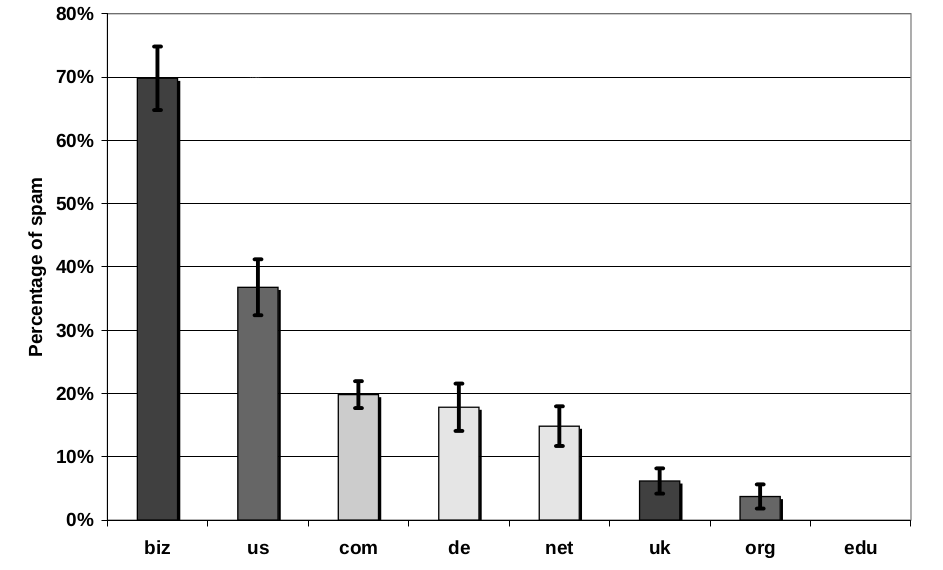
\includegraphics[width=12cm]{immagini/fetterly/fetterly1}
\caption{Occorrenze dello spam classificate per dominio all'iterno del dataset descritto in \cite{Ntoulas:2006:DSW:1135777.1135794}}
\label{fig:fetterly1}
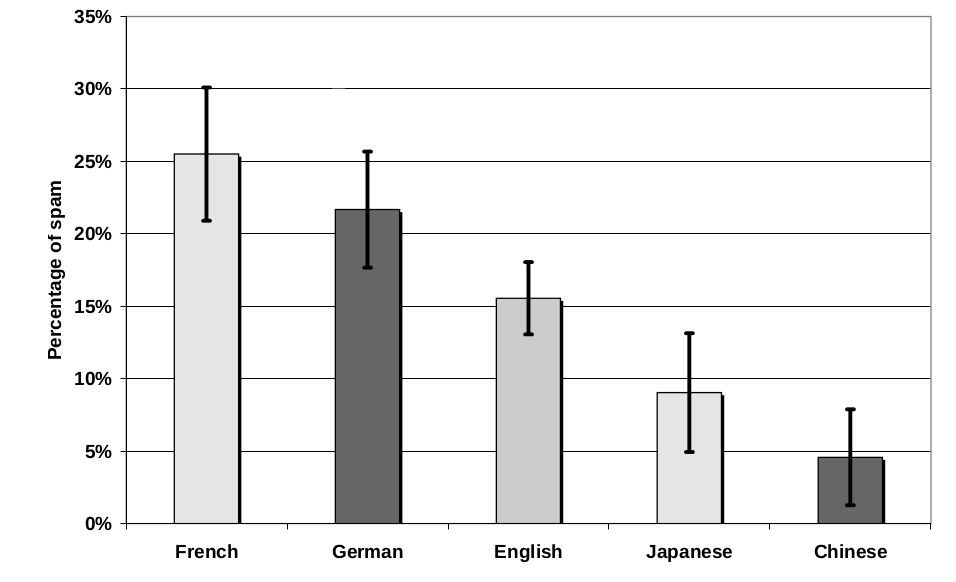
\includegraphics[width=12cm]{immagini/fetterly/fetterly2}
\caption{Occorrenze dello spam classificate per lingua all'iterno del dataset descritto in \cite{Ntoulas:2006:DSW:1135777.1135794}}
\label{fig:fetterly2}
\end{figure}

Una pratica molto comune nel costruire pagine spam è la cosidetta ``Keyword stuffing''. Durante questo processo il contentuto della pagina aumenta con un numero di parole popolari che sono irrilevanti con il resto della pagina. In molti casi per poter aumentare le probabilità di essere messa in cima al rank di molte query, il contenuto di una pagina spam viene aumentato con tante parole estrane all'argomento della pagina. In figura \ref{fig:fetterly3} viene plottato la distribuzione delle parole per ogni pagina del data set. Oltre alla distribuzione delle parole viene raffigurata la percentuale di pagine per ogni range di parole che sono considerate spam. Dal grafico viene notato che la prevalenza di spam è più alta nelle pagine con pmolte parole. Perciò c'è una correlazione tra prevalenza di spam e numero di parole. Il conteggio delle parole da solo non è una buona euristica visto che porta un alto tasso falsi positivi.
\begin{figure}[htbp]
\centering
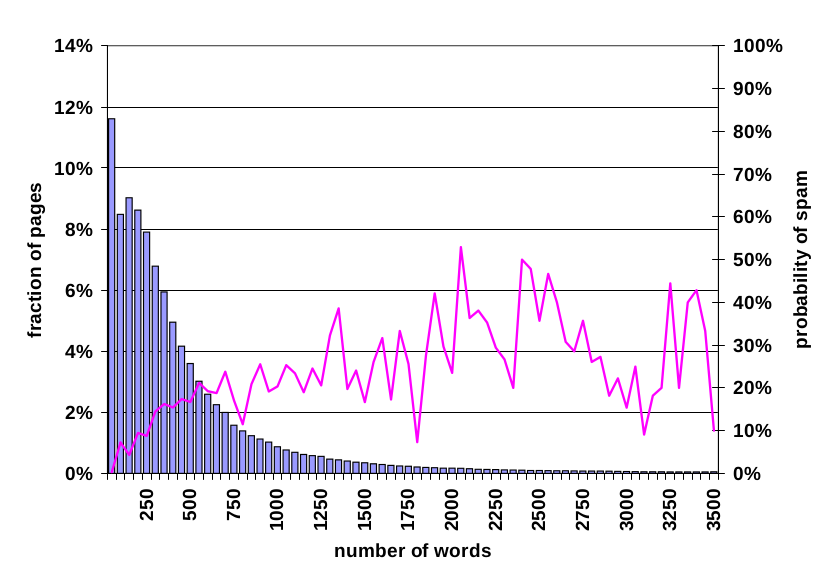
\includegraphics[width=12cm]{immagini/fetterly/fetterly3}
\caption{Prevalenza di spam sulla base del numero di parole per pagina}
\label{fig:fetterly3}
\end{figure}

La tecnica ``Keyword stuffing'' viene utilizzata anche per la costruzione dei titoli delle pagine spam dal momento che alcuni motori di ricerca assegnano un peso maggiore ai termini della query presenti all'interno del titolo della pagina. Il grafico in fugura \ref{fig:fetterly4} rappresenta la distribuzione del numero di parole all'interno dei titoli delle pagine. Come per gli altri grafici viene plottata la rispettiva percentuale di pagine spam. Dal grafico si vede che un'eccesso di parole all'interno del titolo è un indicatore (come per il contenuto della pagina) che una pagina è spam.
\begin{figure}[htbp]
\centering
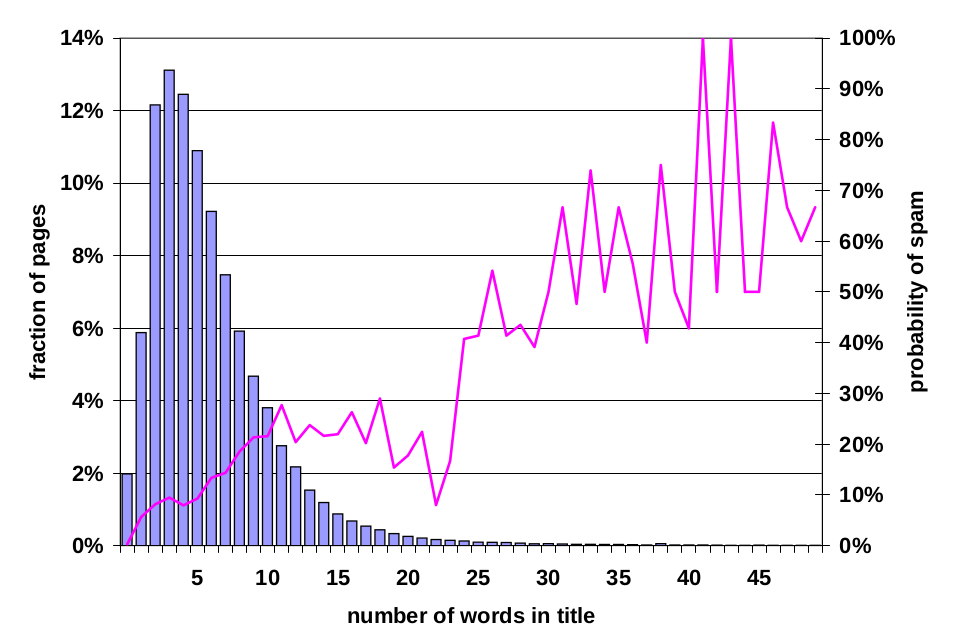
\includegraphics[width=12cm]{immagini/fetterly/fetterly4}
\caption{Prevalenza di spam sulla base del numero di parole all'interno dei titoli delle pagine}
\label{fig:fetterly4}
\end{figure}
Le parole che vengono utilizzate nel processo di ``keyword stuffing'' vengono selezionate casualmente o da un ristretto gruppo di query comuni. Per tentare di esaminare il comportamento con cui vengono selezionate e costruite le frasi vengono esaminate le pagine per  determinare se sono costituite da un eccesso di parole molto comuni. Prima vengono identificate le \textit{n} parole più comuni all'interno del corpus poi viene calcolata, per ogni pagina, la frazione delle parole comuni contenute in ogni pagina. Questo processo viene ripetuto per ogni scelta di \textit{n}. In figura \ref{fig:fetterly9} viene mostrato il grafico per \textit{n=200}. Il grafico è basato sulla frazione di parole di una pagina che sono contenute nell'insime delle 200 parole più comuni nella porzione delle pagine inglesi del data set utilizzato in \cite{Ntoulas:2006:DSW:1135777.1135794}. Il grafico ha una caratteristica gaussiana e suggerisce che la maggior parte delle pagine di spam sono generate tessendo parole da un dizionare con 
una scelta casuale.
\begin{figure}[htbp]
\centering
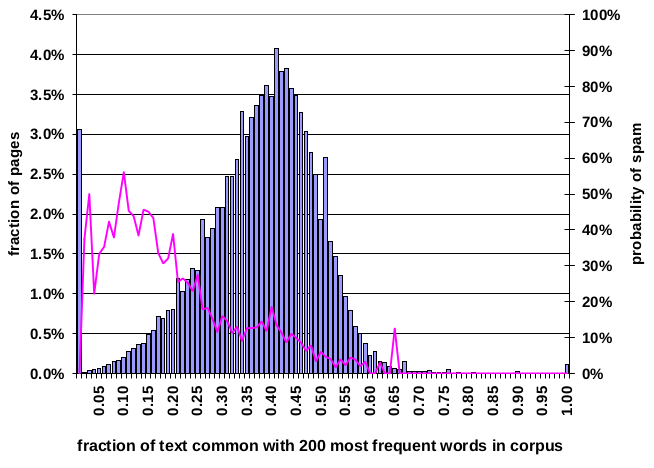
\includegraphics[width=12cm]{immagini/fetterly/fetterly9}
\caption{Prevalenza di spam sulla base della frazione di parole di una pagina che sono tra le 200 piu frequenti parole nel corpus}
\label{fig:fetterly9}
\end{figure}

Un metodo per identificare pagine spam che sono generate automaticamente è descritto in \cite{Fetterly:2005:DPD:1076034.1076066}. Queste pagine spam sono  costruite dinamicamente legando insieme frasi grammaticali ben formate. Le pagine create secondo questo metodo vengono generate al volo e cambiano completamente a ogni download. Queste pagine vengono create per essere indicizzate dalla maggior parte dei motori di ricerca. I link di queste pagine puntano ad altre pagine che sembrano essere su un altro host ma vengono risolte da uno stesso IP. Apparte l'uso di differenti host name ma che in realta corrispondono ad unico host per non creare l'illusione di una struttura nepostica questo meccanismo viene usato anche per eludere le politiche di politeness di un web crawler volte al non sovraccarico di qualsiasi host se tali politiche sono basate sul nome dell'host. Infine generando pagine con frasi formate in modo corretto impediscono agli utenti di individuare l'inganno.

Un altro dato trovato dagli autori per determinare se una pagina è spam riguarda la lunghezza media delle parole delle pagine. Dal dataset preso in considerazione in \cite{Ntoulas:2006:DSW:1135777.1135794} si nota che la distribuzione risultante della lunghezza media delle parole è simile a una gaussiana con moda e mediana corrispondenti a una media di 5.0. La maggior parte delle parole hanno una lunghezza media compresa tra 4.0 e 6.0. Come si nota dal grafico in figura \ref{fig:fetterly5} le parole con lunghezza media 10 sono certamente spam.
\begin{figure}[htbp]
\centering
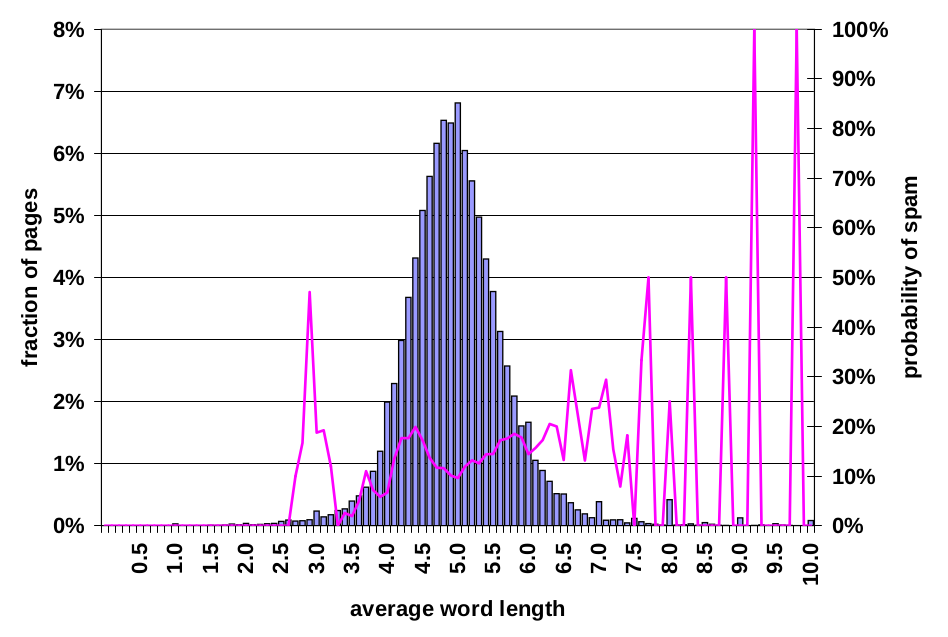
\includegraphics[width=12cm]{immagini/fetterly/fetterly5}
\caption{Prevalenza di spam sulla base della lunghezza media delle parole per pagina}
\label{fig:fetterly5}
\end{figure}

Un'altra proprietà delle pagine web che consente di stimare se una pagina è spam oppure no è la quantita di testo che è contenuta all'interno delle ancore (il tag ``<a>'' delle pagine web). Infatti una pratica comune dei motori di ricerca è considerare il testo delle ancore dei link in una pagina come annotazioni che descrivono il contenuto della pagina che viene puntata dal link. L'idea prinicipale è che se la pagina \textit{a} ha un link alla pagina \textit{b} con testo dell'ancora, ad esempio, ``computer'' allora potremmo concludere che \textit{b} parli di computer, anche se questa keyword non compare all'interno della pagina \textit{b}. Alcuni motori di ricerca tengono conto di questo durante il ranking e potrebbero considerare la pagina \textit{b} come risultato di una query contenente la keyword ``computer''. Sfruttando questo meccanismo alcune pagine di spam vengono create solo per contenere del testo all'interno delle  ancore per valorizzare il ranking di altre pagine. Queste pagine di norma sono 
solo cataloghi di link ad altre pagine. Per capire meglio il fenomeno è stato calcolato la frazione di tutte le parole del testo delle ancore all'interno di una pagina esclusi i markup rispetto al contenuto della pagina. In figura \ref{fig:fetterly6} viene visualizzato il grafico risultante. Si nota che un'alta frazione di testo delle ancore aumenta la probabilita che la pagina sia spam ma usare questa euristica da sola potrebbe portare un alto numero di falsi positivi.
\begin{figure}[htbp]
\centering
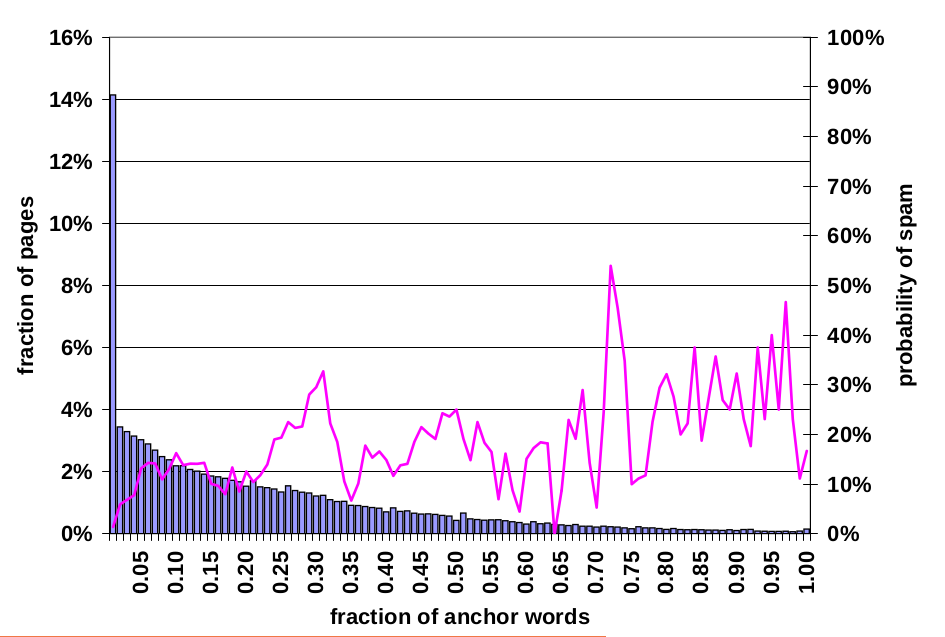
\includegraphics[width=12cm]{immagini/fetterly/fetterly6}
\caption{Prevalenza di spam sulla base della quantità di testo delle ancore delle pagine}
\label{fig:fetterly6}
\end{figure}

Oltre a queste proprietà anche la quantità di contenuto visibile è utile per capire se una pagina è spam. Infatti calcolando la frazione di contentuto visibile all'interno di una pagina: definita come a lunghezza in termini di byte di tutte le parole non di markup diviso l'interna dimensione della pagina, si nota dal grafico in figura \ref{fig:fetterly7} della distribuzione delle frazioni di contenuto visibile che le pagine di spam hanno meno markup delle pagine normali. Questo fa intendere che molte pagine spam hanno il solo scopo di dover essere indicizzate dai motori di ricerca  e non di essere fruite da un utente.
\begin{figure}[htbp]
\centering
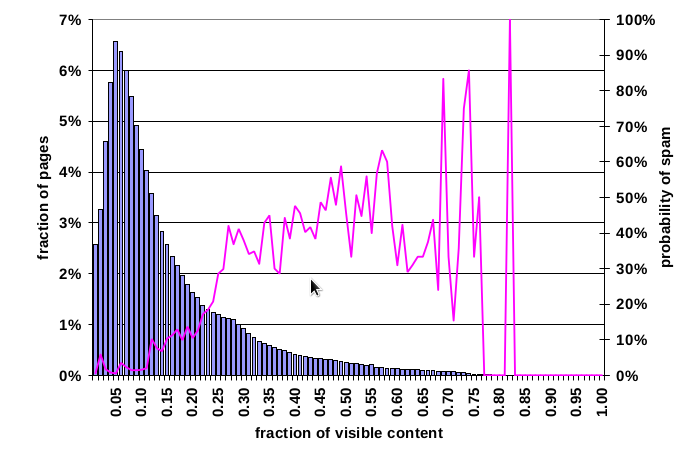
\includegraphics[width=12cm]{immagini/fetterly/fetterly7}
\caption{Prevalenza di spam sulla base della frazione di contenuto visibile}
\label{fig:fetterly7}
\end{figure}

Come detto in precendenza i  motori di ricerca possono dare un maggiore peso a pagine che contengono le keyword contenute nella query più volte all'interno della pagina ad esempio utilizzano come metodo di ranking il ``term-frequency''. Alcune pagine spam per trarre vantaggio da questo meccanismo replicano i contenuti molte volte per aumentare il rank. Per rilevare la rilevare la ridondanza di contenuti (ottenuta dal processo di replica) e perciò stimare se la pagina sia spam, viene calcolato il rapporto di compressione ovvero la dimensione della pagina non compressa divisa per la dimensione della pagina compressa. In figura \ref{fig:fetterly8} viene visualizzato la distribuzione del rapporto di compressione e la likelihood che la pagina sia spam. Dal grafico si nota che quanto più il valore di compressione è elevato molto più probabilmente la pagina può essere considerata spam in particolare  la probabilità che una pagina sia spam risiede sulla parte destra del grafico, il 70 per cento delle pagine con un 
rapporto di compressione maggiore di 4.0 sono giudicate spam. Questo è dovuto al fatto che una compressione su una pagina piena di contenuti ridondanti (spam) sarà più efficace che su una pagina caratterizza da conenuti casuali (non spam). E perciò il rapporto tenderà a crescere quanto più la pagina sarà caratterizzata da contenuti ridondanti.
\begin{figure}[htbp]
\centering
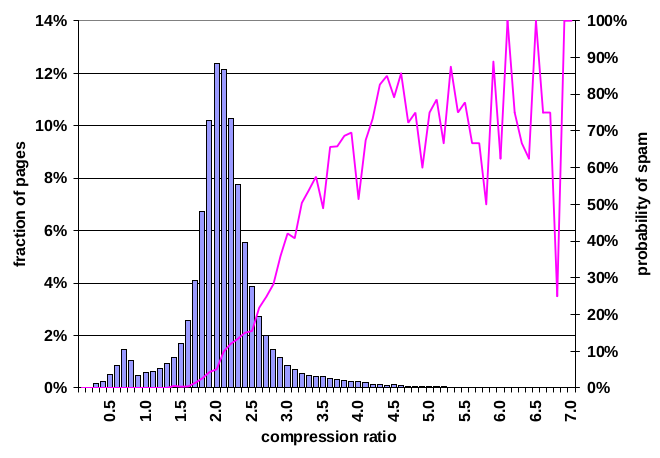
\includegraphics[width=12cm]{immagini/fetterly/fetterly8}
\caption{Prevalenza di spam sulla base del rapporto di compressione}
\label{fig:fetterly8}
\end{figure}

\subsection{Utilizzo di un classificatore per combinare le feature}
Sempre in \cite{Ntoulas:2006:DSW:1135777.1135794} le euristiche vengono combinate considerando il problema di rilevamento dello spam come un problema di classificazione. In questo caso  viene creato un modello di classificazione il quale data una pagina web userà le caratteristiche della pagina in modo tale di classificarla in una delle due classi: spam o non spam. Costruire un classificatore precede una fase di traning durante la quale i parametri del classificatore sono determinati e una fase di testing durante la quale le perfomance del classificatore sono valutate. Per ogni pagina all'interno del dataset viene calcolato il valore di ogni feature (le varie euristiche) e usiamo questi valori per istruire il classificatore. VUsando  un classificatore di tipo ``decision-tree'', l'algoritmo di classificazione funziona come segue: dato un insieme di dati da traning e un insieme di feature l'algoritmo crea un diagramma di flusso come una struttura ad albero. Ogni nodo dell'albero corrisponde al test da valutare 
per una particolare feature mentre ogni arco è un valore di uscita del test ed infine le foglie corrispondono alle classi.  Per applicare l'albero alle pagine viene controllato il valore della proprietà  definita nel nodo radice dell'albero per quella pagina e confrontato con la soglia indicata dai lati uscenti poi si seguono i lati sulla base dei valori ottenuti finche non si arriva ad assegnare la classe per quella pagina. Un esempio del classificatore è rappresentato in figura \ref{fig:fetterly13} Per migliorare il classificatore si possono usare tecniche come bagging o boosting. Le tecninche creano un insieme di classificatori  che vengono combinati.
\begin{figure}[htbp]
\centering
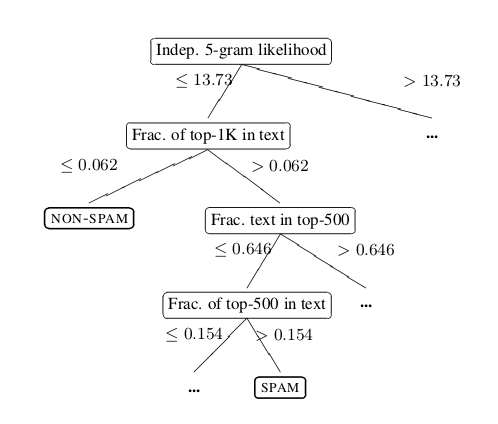
\includegraphics[width=8cm]{immagini/fetterly/fetterly13}
\caption{Esempio di classificatore}
\label{fig:fetterly13}
\end{figure}

\subsection{Modelli dei linguaggi per rilevare lo spam}
In \cite{Martinez-Romo:2009:WSI:1531914.1531920} vengono proposte nuovi tipi di feature per rilevare lo spam e vengono definiti dei modelli dei linguaggi per analizzare le sorgenti estratte da ogni sito in un dataset.  Questo metodo di rilevamento delle pagine web spam fa uso di feauture basate su contenuto e struttura dei link in modo combinato per rilevare differenti tipi di web spam. Viene creato un modello del linguaggio per ogni sorgente e calcolato quanto sono differenti i due modelli  da ogni altro modello. Le sorgenti di informazioni usate sono: 
\begin{itemize}
\item testi delle ancore e testo vicino alle ancore della pagine sorgente
\item titolo e contenuto della pagina obbiettivo dello spam
\end{itemize}
Viene utilizzata la Kullback-Leibler Divergence (KLD) per misurare la divergenze tra le distribuzioni di probabilità dei termini di due documenti. La KLD viene applicata a unità di testo della pagina sorgente e di quella linkata. Infatti a Kullback-Leibler (KL), una misura  asimmetrica della divergenza la quale misura quanto male una distribuzione di probabilità \(M_q\) riesce a modellare \(M_d\).
\begin{equation}
KLD(T_1||T_2) = \sum_{t \in T_1} P_{T_1}(t) \log \frac{P_{T_1}(t)}{P_{T_2}(t)}
\label{eqn:kld}
\end{equation}
dove in \ref{eqn:kld} \(P_{T_1}(t)\) è la probabilità del termine \textit{t} nella prima unità di testo e \(P_{t_2}(t)\) è la probabilità del termine texit{t} nella seconda unità di testo. In basso sono rappresentati due esempi di KLD applicata tra il testo delle ancore della pagina sorgente e i titoli delle pagine puntate dai i link (esempio preso da WEBSPAM-UK2006).
\begin{lstlisting}[frame=trbl,postbreak=\space, breakindent=5pt, breaklines]
KLD(Free Ringtones || Free Ringtones for Your Mobile Phone from PremieRingtones.com) = 0.25

KLD(Best UK Reviews || Findabmw.co.uk - BMW Information Resource) = 3.89
\end{lstlisting}
Per la determinazione determinare se una pagina è spam viene provato a trovare una relazione tra due pagine collegate sulla base del loro valore di divergenza. I valori sono ottenuti calcolando le divergenze con KLD tra una o più sorgenti di informazioni da ogni pagina. In particolare si usano tre tipi di informazione di una pagina sorgente: testo delle ancore, testo intorno alle ancore, termini nell'URL. Sono utilizzate tre tipi di informazione per la pagina che viene linkata dalla pagina sorgente: titolo, contenuto della pagina, meta tag. La combinazione di queste feature possono essere usate per determinare la divergenza tra due pagine. Le feature sono descritte di seguito:
\begin{itemize}
\item testo delle ancore - contenuto. Quando una pagina collega un'altra pagina questa ha solo un modo per convincere l'utente di visitare la pagina collegata, mostrare in maniera concisa le informazione relative alla pagina collegata. Perciò una grande divergenza tra questi due pezzi di testo mostra una chiara evidenza di spam. In figura \ref{fig:martinez1} è mostrato la divergenza KL tra le sorgenti di informazione, come si vede la curva delle pagine normali è più compatta delle spam. Ma da sola questa feature non è una buona misura.
\begin{figure}[htbp]
\centering
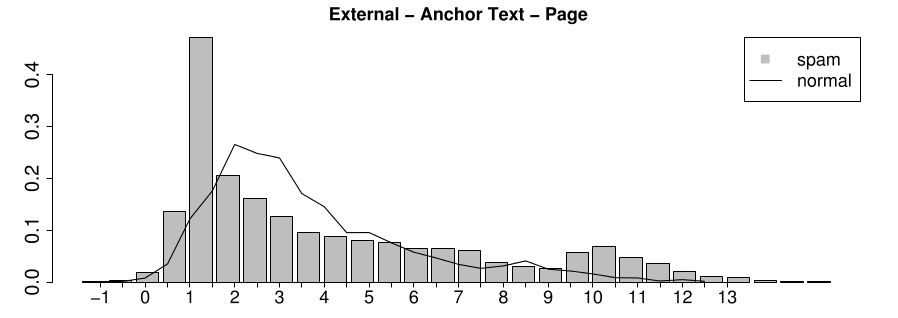
\includegraphics[width=12cm]{immagini/martinez/martinez1}
\caption{Istogramma della divergenza KL tra testo delle ancore e il contenuto della pagina puntata basato sul dataset WEBSPAM-UK2006 utilizzato in \cite{Martinez-Romo:2009:WSI:1531914.1531920}}
\label{fig:martinez1}
\end{figure}

\item testo vicino alle ancore - contenuto. Alcune volte il testo delle ancore è un valore poco descrittivo per ovviare al problema viene usato il testo che circonda le ancore. Nell'esperimento vengono utilizzate 7 parole per lato. Il risultato è che questa feature riesce meglio a rilevare lo spam. In figura \ref{fig:martinez2} viene mostrato che le pagine spam hanno alti valori di divergenza mentre le normali sono concentrate intorno \(KL \approx  2.5\).
\begin{figure}[htbp]
\centering
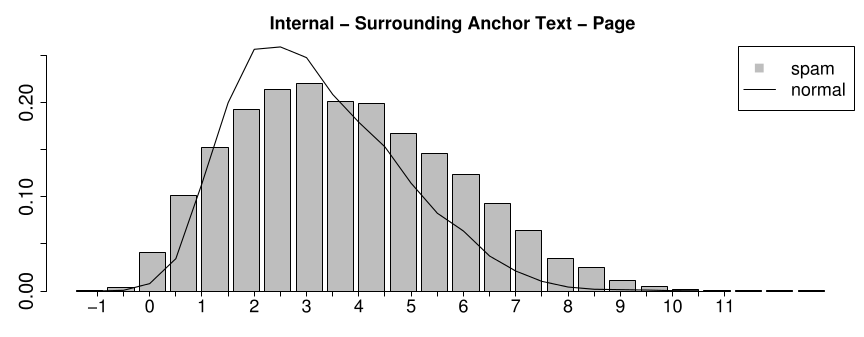
\includegraphics[width=12cm]{immagini/martinez/martinez2}
\caption{Istogramma della divergenza KL tra testo intorno alle ancore e il contenuto della pagina puntata basato sul dataset WEBSPAM-UK2006 utilizzato in \cite{Martinez-Romo:2009:WSI:1531914.1531920}}
\label{fig:martinez2}
\end{figure}

\item termini nell'URL - contenuto. Negli URL ci possono essere informazioni che descrivono bene la pagina di destinazione. I motori di ricerca danno molta importanza agli URL per questo un metodo di spam è creare URL come \url{www.domain.com/viagra-youtube-free-download-poker-online.html} e se visitiamo la pagina questa è magari uno store online. Questa è una delle tecniche per fare spamming. Perciò vengono prelevati i termini più rilevanti da un URL in modo tale da calcolarne la divegenza col contenuto della pagina di destinazione. La misura finale si vede in figura \ref{fig:martinez3} che mostra una grande differenza tra l'istogramma delle pagine normali con quello delle pagine spam.
\begin{figure}[htbp]
\centering
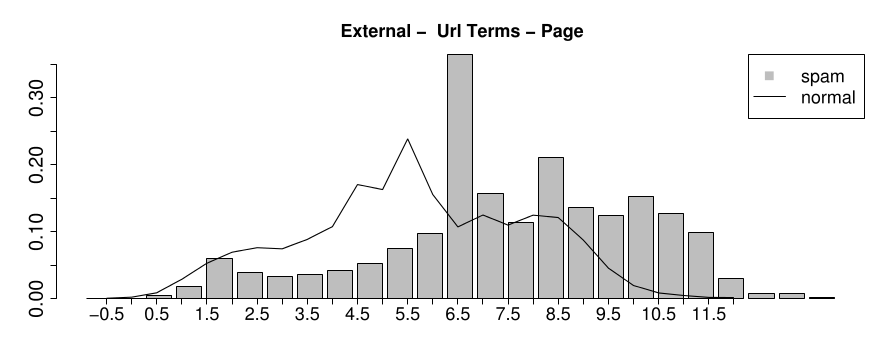
\includegraphics[width=12cm]{immagini/martinez/martinez3}
\caption{Istogramma della divergenza KL tra termini degli URL e il contenuto della pagina puntata basato sul dataset WEBSPAM-UK2007 utilizzato in \cite{Martinez-Romo:2009:WSI:1531914.1531920}}
\label{fig:martinez3}
\end{figure}

\item testo delle ancore - titolo. Queste due feature sono molto simili inquanto descrivono la pagina con poche parole. Ma la prima può essere scritta anche da chi non è il proprietario della pagina destinazione.  In figura \ref{fig:martinez4} notiamo che questa feature da sola non descrimina bene i due tipi di pagine ma è abbastanza efficace utilizzata in congiunzione con altre feature.
\begin{figure}[htbp]
\centering
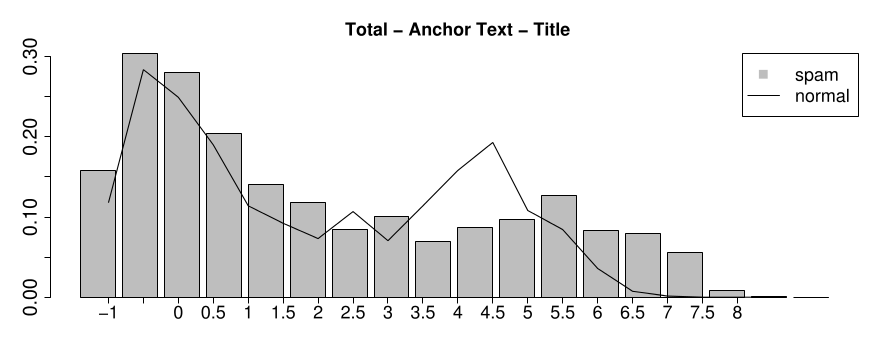
\includegraphics[width=12cm]{immagini/martinez/martinez4}
\caption{Istogramma della divergenza KL tra testo delle ancore e titolo della pagina puntata basato sul dataset WEBSPAM-UK2007 utilizzato in \cite{Martinez-Romo:2009:WSI:1531914.1531920}}
\label{fig:martinez4}
\end{figure}

\item testo intorno alle ancore - titolo. Dal grafico in figura \ref{fig:martinez5} vediamo che rispetto alla feature precedente questa rileva meglio lo spam infatti molti valori di spam sono concentrati per valori di \(KL > 3\).
\begin{figure}[htbp]
\centering
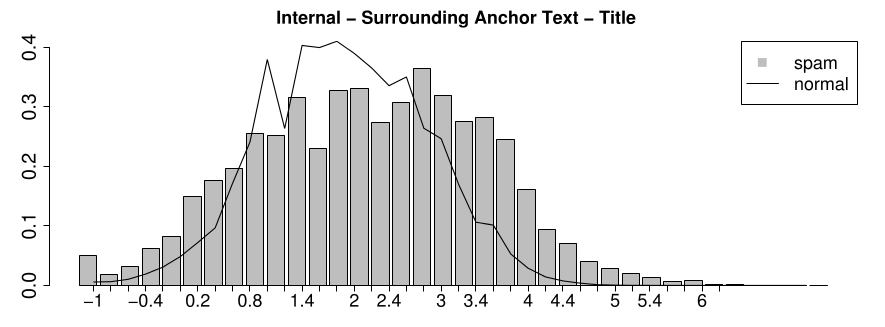
\includegraphics[width=12cm]{immagini/martinez/martinez5}
\caption{Istogramma della divergenza KL tra testo intorno alle ancore e titolo della pagina puntata basato sul dataset WEBSPAM-UK2006 utilizzato in \cite{Martinez-Romo:2009:WSI:1531914.1531920}}
\label{fig:martinez5}
\end{figure}

\item termini nell'URL - titolo. Se bene nella precendente feature la sorgente di informazione della pagina sorgente poteva essere generata da un'altra persona in questo caso entrambe le sorgenti sono generate dal proprietario della pagina. Questo dovrebbe fornire coerenza tra le due sorgenti. In figura \ref{fig:martinez6} è evidente che la curva delle pagine spam è più compatta della della curva dell'istogramma delle pagine normali.
\begin{figure}[htbp]
\centering
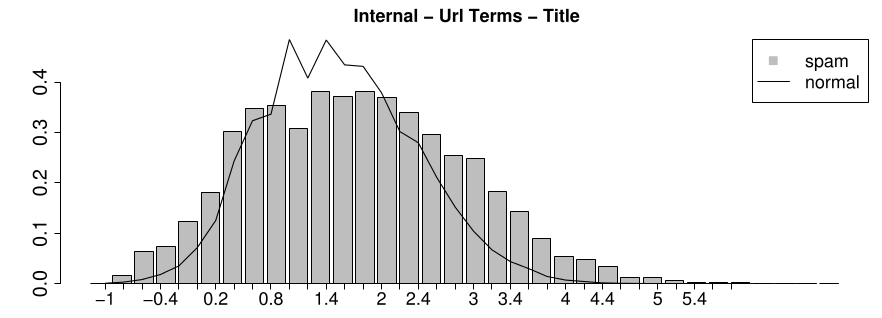
\includegraphics[width=12cm]{immagini/martinez/martinez6}
\caption{Istogramma della divergenza KL tra termini nell'URL e titolo della pagina puntata basato sul dataset WEBSPAM-UK2006 utilizzato in \cite{Martinez-Romo:2009:WSI:1531914.1531920}}
\label{fig:martinez6}
\end{figure}

\item titolo - contenuto. I motori di ricerca danno un peso maggiora ai termini dell'URL di una pagina e del titolo. GLi spammer perfezionano i loro processi in modo tale da impostare termini chiave in queste sorgenti che vengono create. In figura \ref{fig:martinez7} è rappresentata la divergenza tra le due distribuzioni. Questa misura consente di rilevare i casi di spam quando non vi è nessuna relazione tra il titolo e il contenuro della pagina dello stesso sito.
\begin{figure}[htbp]
\centering
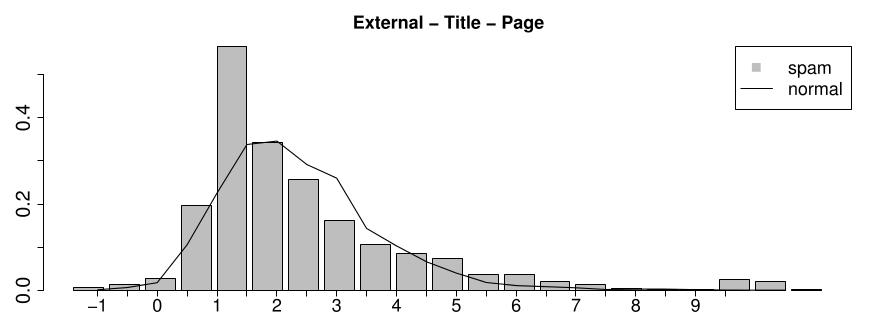
\includegraphics[width=12cm]{immagini/martinez/martinez7}
\caption{Istogramma della divergenza KL tra titolo  e contenuto della pagina basato sul dataset WEBSPAM-UK2006 utilizzato in \cite{Martinez-Romo:2009:WSI:1531914.1531920}}
\label{fig:martinez7}
\end{figure}

%correggere
\item meta tag. Sono stati usati per calcolare la divergenza con altre sorgenti di informazioni della pagina sorgente come il testo delle ancore e il testo intorno alle ancore e per calcolare la divergenza con sorgenti della pagina destinazione come il contenuto o i temini dell'URL. In figura \ref{fig:martinez8} viene visualizzata la differenza tra le due distribuzioni.
\begin{figure}[htbp]
\centering
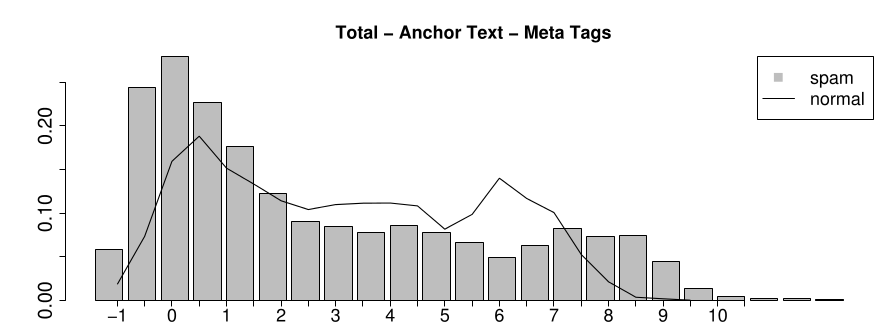
\includegraphics[width=12cm]{immagini/martinez/martinez8}
\caption{Istogramma della divergenza KL tra testo delle ancore  e i meta tag della pagina basato sul dataset WEBSPAM-UK2006 utilizzato in \cite{Martinez-Romo:2009:WSI:1531914.1531920}}
\label{fig:martinez8}
\end{figure}
\end{itemize}
Oltre alle feature descritte: testo delle ancore (A), termini nell'URL (U), testo intorno alle ancore (A), per le pagine sorgenti possono essere definite altre feature combinandole tra di loro: testo delle ancore e termini nell'URL (AU), testo intorno alle ancore e URL (SU) mentre per quanto riguarda le pagine destinazione possono essere usate le stesse sorgenti cioè contenuto della pagina (P), titolo (T), metatag (M). Per maggiori dettagli \cite{Martinez-Romo:2009:WSI:1531914.1531920}.

Queste feature possono essere usate per istruire un classificatore e identificare le pagine spam.

\subsection{L'algoritmo WITCH}
Nel 2008 in \cite{Abernethy:2008:WSI:1451983.1451994} viene presentato  l'algoritmo WITCH (Web Spam Identification Through Content and Hyperlinks), un'algoritmo ibrido che utilizza sia il contenuto della pagina che la struttura dei link per identificare le pagine spam. Come descritto in precedenza nel sotto capitolo \ref{subsec:Feature} e in particolare in \cite{Ntoulas:2006:DSW:1135777.1135794}, le pagine spam e non spam hanno differenti proprieta le quali possono essere sfruttate per costruire un classificatore. L'algoritmo WITCH oltre alle feature standard descritte in precedenza (vedi il sotto capitolo: \ref{subsec:Feature})per identificare lo spam analizza la struttura dei collegameti tra le pagine. In particolare viene istruit un classificatore lineare nello spazio delle feature usando la SVM (Support Vector Machine) come funzione obbiettivo. I collegamenti tra le pagine sono utilizzati in modo da regolarizzare il grafo che produce una predizione che varia leggermente tra le pagine dei link. Il risultato è che il metodo SVM associato alla regolarizzazione del grafo è efficiente per il rilevamento di web spam. 

